\chapter{Control system architecture components}
In this section, we provide a detailed description of the individual
control system components of this architecture.

\section{3D-printed prosthetic hand}
Many open-source 3D-printable prosthetic hands are available. All of
our prosthesis parts are defined in stereolithography (STL) files
\cite{STL} with different designs that can be modified for the
best-fitting model for each different user.  Armed with those STL
files, the 3D printer can generate a prosthetic hand with diverse
sizes for different people who need it. For the experiments, an
open-source design was adopted and printed with a 3D printer, which is
easily modified in the future for each user's needs.

In our prosthesis prototype, five MG996R servo motors with a maximum
stall torque of 11 kgf·cm powered by 6V are used as actuators, one for
each finger \cite{3D1}. The motors are controlled by an Arduino Mega
Atmel 8-bit AVR microcontroller. When the EMG sensors detect a muscle
contraction, the microcontroller controls individual servo motors to
control individual fingers in real-time through the decision-making
process. The printed 3D prosthetic hand is shown in Fig. \ref{hand}.

% \begin{figure}[h]
%   \centering
% %   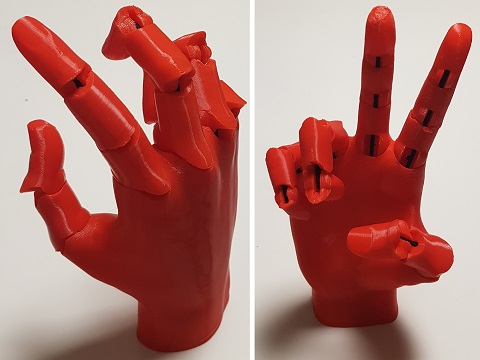
\includegraphics[width=3.0in]{Figures/3dhand3.jpg}
%   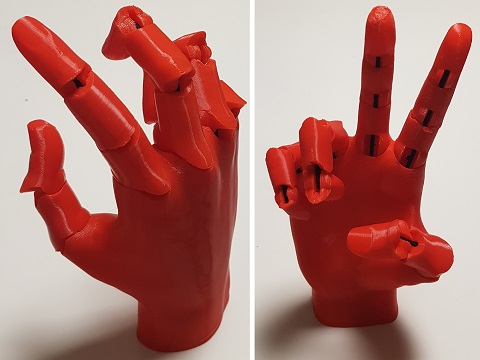
\includegraphics[.9\textwidth]{Figures/3dhand3.jpg}
%   \caption{3D-printed prosthetic hand}
%   \label{hand}
% \end{figure}

\singlefigure[.9\textwidth]{hand}{3dhand3.jpg}{3D-printed prosthetic hand}{3D-printed prosthetic hand}


%% Electromyography Signal

\section{Electrical biosignal sensors}

\subsection{Electromyography sensors}

To detect and measure the electrical activity produced by muscle
contraction, the electrodiagnostic technique is considered as an input
for the decision-making process. The MyoWare Muscle Sensor is used,
which is designed for microcontroller applications \cite{myo} with the
dimension of 52.3x20.7mm.  It needs a voltage power between 2.9-5.7 V
with a maximum current of 14mA. As shown in Fig. \ref{myo}, the sensor
can measure the muscle's electrical potential with three electrodes
when the sensor board is placed at the skin above the targeted muscle.

% \begin{figure}[h]
%   \centering
%   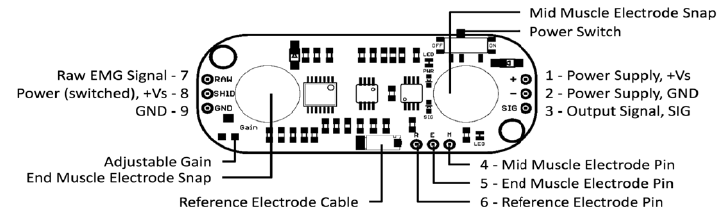
\includegraphics[width=3.4in]{Figures/myosensor.png}
%   \caption{The layout of the MyoWare Muscle Sensor (AT-04-001)}
%   \label{myo}
% \end{figure}

\singlefigure[.9\textwidth]{myo}{myosensor.png}{The layout of the MyoWare Muscle Sensor (AT-04-001)}{The layout of the MyoWare Muscle Sensor (AT-04-001)}

\subsection{EMG signal processing}

The MyoWare Sensor can detect envelope EMG and raw EMG with the
voltage signal difference between the central muscle electrode and the
reference electrode. The sensor generates the envelope signal, which
is amplified, rectified, and integrated within the sensor transducer,
as shown in Fig. \ref{signal}. The signal amplitudes are translated
through the microcontroller's analog-to-digital converter (ADC), and
are then utilized as features to select human behaviors at the
decision-making process.

% \begin{figure}[h]
%   \centering
%   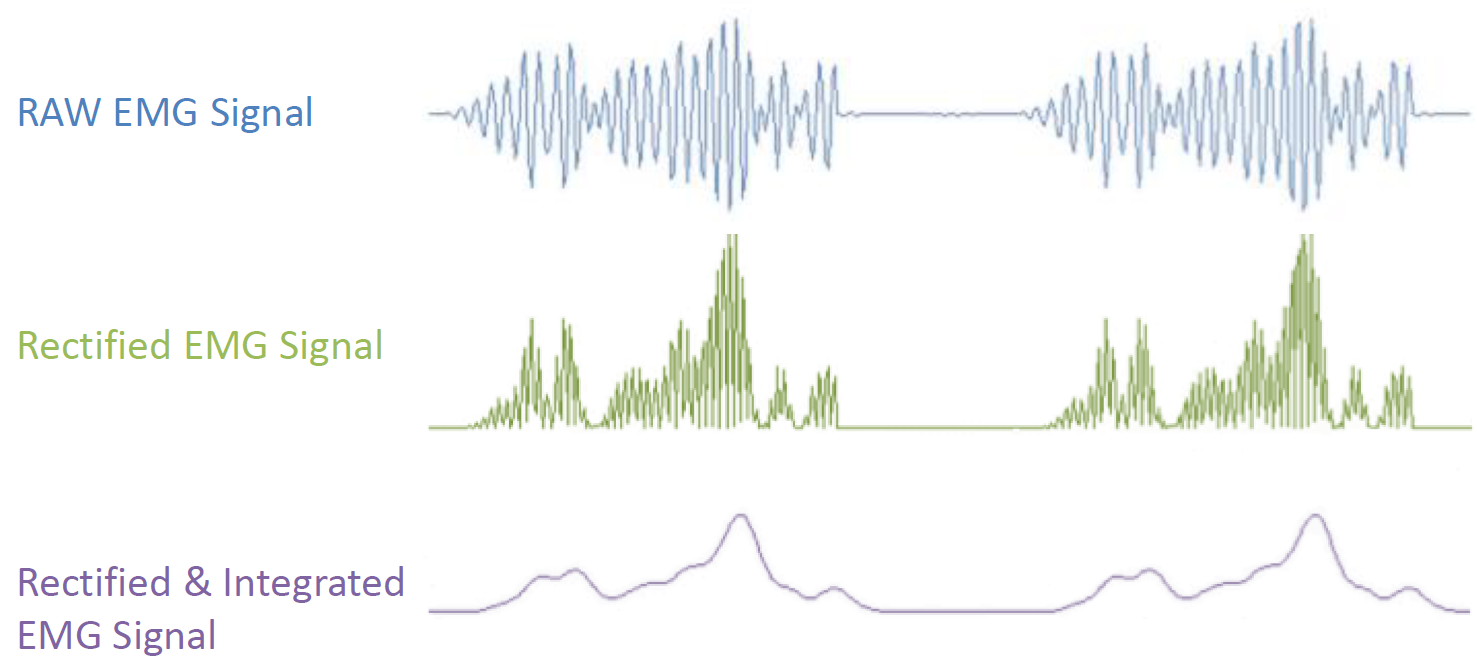
\includegraphics[width=3.2in]{Figures/signals.png}
%   \caption{An example of EMG signals processing}
%   \label{signal}
% \end{figure}

\singlefigure[.9\textwidth]{signal}{signals.png}{An example of EMG signals processing}{An example of EMG signals processing}




\subsection{Electroencephalogram sensors}
Electrodes placed on your scalp detect tiny electrical charges that
result from the activity of your brain cells to identify and measure
the electrical activity produced by irregularities in your brain
signals or electrical activity of your brain.
The electrodiagnostic approach is used as a source of information
for decision-making.
The Muse S brain sensing headband is used, which is designed for
a multi-sensor brain-computer interface headband that can give you
real-time feedback on your brain waves.

\subsection{EEG signal processing}
The Muse S can detect signals from TP9, AF7, AF8, TP10 in the
international standard EEG placement system. According to the technical manual \cite{[???}, Muse S receives a raw signal ranging from 0 to 1682 microvolts (V), which can represent the raw data of each sensor. Fast Fourier Transform (FFT) of raw data is used to generate discrete frequency values on the log scale. The frequency bands of the brain waves can be determined using a spectrum of discrete frequency data: Gamma (30-44 Hz), Beta (13-30 Hz), Alpha (7.5-13 Hz), Theta (4-8 Hz), and Delta (1-4 Hz). Based on the Power Spectrum Density (PSD) log of EEG data for each channel, this absolute band power is utilized as a function of selecting human behavior in the decision-making process.
% PICTURE
% PICTURE
% PICTURE
\section{Self-training user-customized control software}

In our software designed to train the user's prosthetic hand, all the
magnitude of the envelope signals, generated by 3 channel EMG sensor
signals, were transferred to the Arduino platform. The microcontroller
can read and record all the sensor data as a user history to train
each behavior into the machine. In the trained device, these three
matrix values contain sensor values (0-1000) as inputs, which are used
to produce prosthetic hand behavior decision-making in real-time.  The
training function procedure and the actual operation function
procedure are presented in Algorithm \ref{alg:sysArch}.

% Algorithm
\begin{algorithm}
\caption{System architecture}
\label{alg:sysArch}
\begin{algorithmic}[1]
\Procedure{Training}{}

\State \textit{y.append(CustomGesture)}
\Comment{custom new gesture}
\For {$i=y_{0}$ to $y_{max}$}
    \For {$j=0$:$T$}
        \State $ \textit{$X_{j}^i$} \gets \textit{readSensors()}$
        \EndFor
    \EndFor
\State \textit{clf.fit(X, y)}
\EndProcedure

\Procedure{Movements}{}
\While{$r\not=0$}
\State \textit{ $Gesture = predict(readSensors()) $}
\State \textit{ $MotorController(Gesture, servoMotors())$ }
\EndWhile\label{endwhile}
\EndProcedure
\end{algorithmic}
\end{algorithm}

To train the model, a user's custom gesture is appended (as many as
desired). Each $y$ contains each custom gesture per $T$ iterations,
and each sensor's value is recorded in $X$ for the classification.
The motor outputs provided to move each finger by motor controller
depend on the prediction for the user's specific gesture.

A support vector machine (SVM) \cite{ML1}\cite{ML2} supervised
learning methods, is applied to the prosthetic hand's behavior
classification, with a radial basis function (RBF) kernel. The radial
basic function network has the advantage of solid tolerance to input
noise and is well suited for designing flexible control systems
\cite{RBFAdv}. This gesture classification uses multiple EMG sensors
as input matrix $X$, and the output matrix $y$ consists of each
different individual intended gesture.

The equation \eqref{kernel} defines the radial basis function kernel
for two different inputs $X$ and $X'$, designated as feature vectors,
which is the factor to predict purposing action with trainable
high-performance accuracy.
\begin{equation}
K(X,X') = \exp(-\frac{\lVert X - X' \rVert^2}{2\sigma^2})
\label{kernel}
\end{equation}

The squared Euclidean distance between the two feature vectors is
shown in $\lVert X - X' \rVert^2$.  The $\sigma$ worked as a parameter
condition.


%%% NO NEED TO EXPLAIN
The artificial neural network interpretation of SVMs using radial basis function kernel to train the prosthesis is demonstrated in Fig. \ref{RBF}.

%% RBF figure
\begin{figure}[htp]
% \begin{figure}[t]
\centering
\begin{tikzpicture}[
plain/.style={
  draw=none,
  fill=none,
  },
net/.style={
  matrix of nodes,
  nodes={
    draw,
    circle,
    inner sep=8.5pt
    },
  nodes in empty cells,
  column sep=0.6cm,
  row sep=-11pt
  },
>=latex
]
\matrix[net,row sep=0em, column sep=3em] (mat)
{
             &           \\
  |[plain]|  & |[plain]| &  &         \\
             &           \\
  |[plain]|$\vdots$ & |[plain]|$\vdots$ &  &       \\
             &           \\
};
\foreach \ai in {1,3,5}
  {\foreach \aii in {1,3,5}
    \draw[->] (mat-\ai-1) -- (mat-\aii-2);
}
\foreach \ai in {1,3,5}
  {\foreach \aii in {2,4}
    \draw[->] (mat-\ai-2) -- (mat-\aii-3)node(){$\sum$};
}
\draw[->] (mat-2-3) -- (mat-2-4)node(){$y_1$};
%\draw[->] (mat-2-5)node(){$t_i$} -- (mat-2-4);
 
\draw[->] (mat-4-3) -- (mat-4-4)node(){$y_k$};
% \draw[->] (mat-4-5)node(){$t_k$} -- (mat-4-4);

\node(x1) at (mat-1-1){$x_1$}; \node(s1) at (mat-1-2){$\sigma_1$};
\node(x1) at (mat-3-1){$x_2$}; \node(s2) at (mat-3-2){$\sigma_2$};
\node(x1) at (mat-5-1){$x_i$}; \node(s3) at (mat-5-2){$\sigma_3$};
\end{tikzpicture}
\caption{Radial basis function model}
\label{RBF}

\end{figure}

The support vector classification implementation is tuned with
regularization parameter $C = 2.5$, and the kernel coefficient for RBF
$\gamma = 0.01$ as the best fit.